\section{Nearest Neighbor and LSH}

\begin{frame}{Nearest Neighbor}
\begin{itemize}
    \item Nearest Neighbor 是一种非参数化模型。(数据集就是参数)
    \item 直接用遍历所有点的方式找到邻居的方法非常耗时,希望有一种数据结构能够高效返回近似最近邻
    \item LSH algorithm
\end{itemize}
\end{frame}

\begin{frame}{LSH}
    Formally, 我们希望解决以下最近邻高效查找问题:
    \begin{block}{$\epsilon$-NNS Problem}
        给定在 normed space $\ell_p^{d}$ (距离定义为$\ell_p$-norm的$d$维空间) 中的点集$P$ ,处理$P$使任给查询点$q$,数据结构能高效返回一个点$p \in P$ 满足 $d(q, p) \leqslant (1+\epsilon) d(q, P)$,其中$d(q, P)$是$q$到$P$中最近点的距离。
    \end{block}
    思想:
    \begin{itemize}
        \item 使用 hash 方法,希望距离近的点更有可能被分在同一组中。(即,希望同一个hash table组中包含许多相互靠近的点,但也可能包含距离较远的点)
        \item 单独一个hash table随机性太大,因此创建一个family of hash functions。
    \end{itemize}
\end{frame}

\begin{frame}{LSH Family}
    \begin{block}{LSH Family: $(R, cR, P_1, P_2)$-sensitive}
        一个family $H$ 被称作是$(R, cR, P_1, P_2)$-sensitive 的,若对任意两点$p, q \in \mathbb{R}^{d}$,有:
        \begin{itemize}
            \item 若$d(p, q) \leq R$,则$\Pr_{h \in H}[h(p) = h(q)] \geq P_1$
            \item 若$d(p, q) \geq cR$,则$\Pr_{h \in H}[h(p) = h(q)] \leq P_2$
        \end{itemize}
        其中对$h$从$H$中均匀随机选择 (uniformly at random)。
    \end{block}
    \begin{itemize}
        \item 若希望能有区分度,要求$P_1 > P_2$。
        \item 思想:如果两个点很近 ($d \leqslant R$),则$H$中有很多hash函数能够将这两个点映射到同一个值;如果两个点很远 ($d \geqslant cR$),则$H$中很少的hash函数能够将这两个点映射到同一个值。
    \end{itemize}
\end{frame}

\begin{frame}{Example 1: LSH for Hamming Distance in $\left\{ 0, 1 \right\}^{d} $ space}
    定义 LSH family 为 
        \[
            H = \left\{ h_i : \left. \left\{ 0, 1 \right\} ^{d} \to \left\{ 0, 1 \right\} \right| h_i(x) = x_i, \forall i \in [d] \right\} 
        \]
        注意到
    \begin{itemize}
        \item 若$d_H(x, y) \leqslant R$,则$x, y$最多有$R$位不同,因此至少有$d-R$个hash函数能够将$x, y$映射到同一个值$\Rightarrow \Pr_{h \in H}[h(p) = h(q)] \geq 1-\frac{R}{d} = P_1$。
        \item 若$d_H(x, y) \geqslant cR$,则$x, y$至少有$cR$位不同,因此至多有$d-cR$个hash函数能够将$x, y$映射到同一个值$\Rightarrow \Pr_{h \in H}[h(p) = h(q)] \leq 1- \frac{cR}{d} = P_2$。
    \end{itemize}
    因此,family $H$是$(R, cR, 1-\frac{R}{d}, 1-\frac{cR}{d})$-sensitive的。
    
\end{frame}

\begin{frame}{Example 2: LSH for $\ell_p$ Distance in $\mathbb{R}^{d} $ space ($p \in (0, 2]$)}
    定义 LSH family 为 
        \[
            H = \left\{ h_{r, b} : \left. \mathbb{R}^{d} \to \mathbb{R} \right| h_{r, b}(x) = \left\lfloor \frac{r \cdot x + b}{w} \right\rfloor \right\}\tag{2}
        \]
        其中$r \sim p-\text{stable Distribution}$, $b \sim \text{Uniform}[0, w)$。

    \begin{itemize}
        \item 对 $p=1$,stable distribution是 Cauchy distribution:
        \[
            f_1(x) = \frac{1}{\pi(1+x^2)}
        \]
        \item 对 $p=2$,stable distribution是 Gaussian distribution:
        \[
            f_2(x) = \frac{1}{\sqrt{2\pi}} \exp(-\frac{x^2}{2})
        \]
        \item 可以证明,按(2)式定义的family满足$(R, cR, P_1, P_2)$-sensitive。
    \end{itemize}
    
\end{frame}

\begin{frame}{Example 2: LSH for $\ell_p$ Distance in $\mathbb{R}^{d} $ space ($p \in (0, 2]$)}
    对 $p$-stable distribution 的更详细解释:

    \begin{itemize}
        \item  $p$-stable distribution 定义为
        \begin{center}
            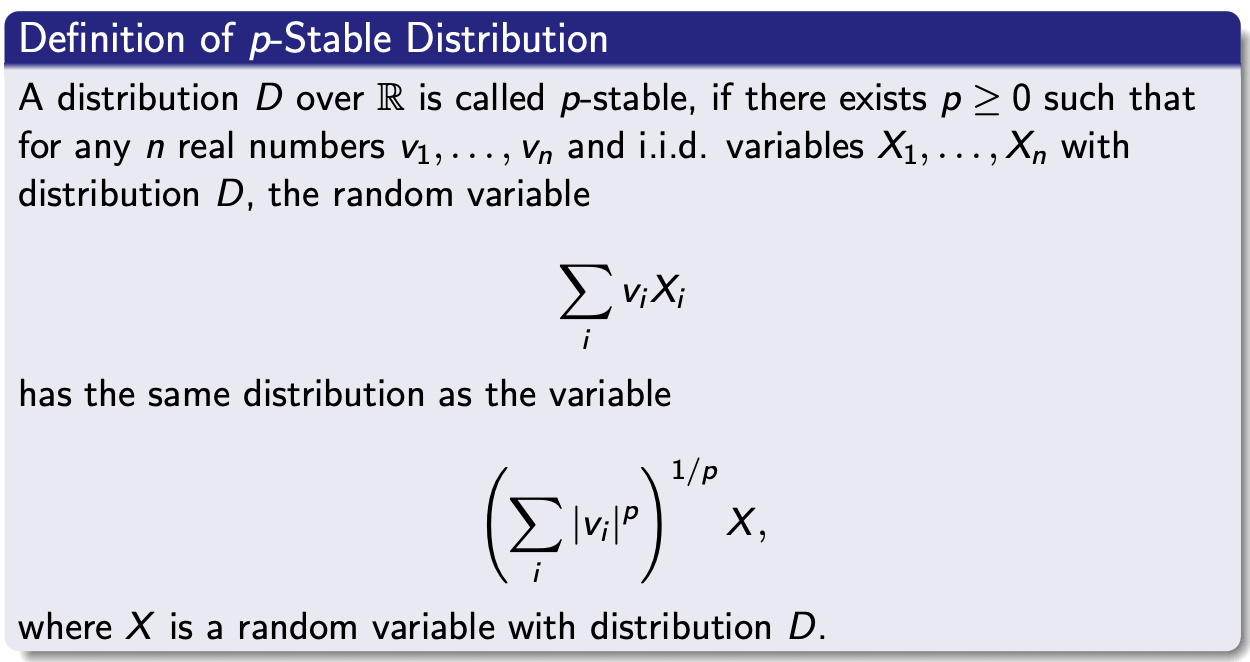
\includegraphics[width=0.6\textwidth]{assets/psd.png}
        \end{center}
        \item 按照如上定义,在计算 $\Pr_{h \in H}[h(p) = h(q)]$ 时遇到的 $r \cdot (p-q)$ 的分布等于 $\left\| p-q \right\|_p \cdot r_1 $,其中$r_1$ 服从一维 $p$-stable distribution。这样$\Pr_{h \in H}[h(p) = h(q)]$容易计算。
    \end{itemize}
    
\end{frame}

\begin{frame}{LSH Algorithm}
    算法:
    \begin{center}
        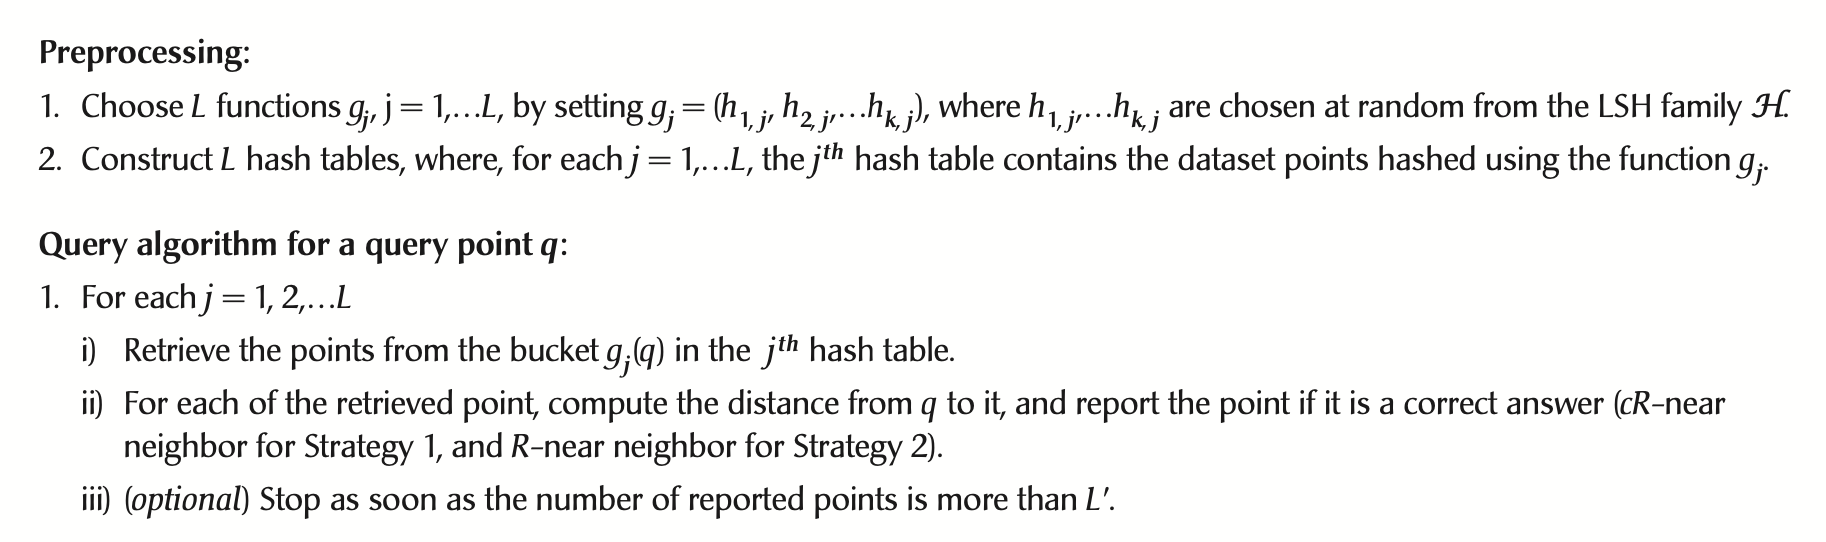
\includegraphics[width=0.95\textwidth]{assets/lsh.png}
    \end{center}
    注意:$g_j(p) = (h_{j_1}(p), h_{j_2}(p), \cdots, h_{j_k}(p))$是新的hash function,通过组合LSH family中若干随机性比较大的hash function组成。
    在Yang Yuan的版本中,$L' = 2L+1$,Yang Yuan证明了只用查找最多$2L+1$个点就一定能保证report一个$cR$-near的点。
\end{frame}

\begin{frame}{LSH Algorithm Analysis}
    \begin{block}{Theorem}
        使用以上算法查找$q$的近邻点,若存在$p^{*} \in P$使 $p^{*} \in B(q, R)$, 则以上算法返回一个与$q$ $cR$-near的点的概率至少为$\frac{1}{2} - \frac{1}{\mathrm e }$   .
    \end{block}
    证明思路:
    \begin{itemize}
        \item 所有与$q$至少有一个$g_j$相等、且不与 $q$ $cR$-near的点$p$ (换句话说,就是至少有一个hash表,$q$和$p$在同一个桶中,因为只有这样算法才可能report 这个点$p$) 的个数$\leqslant 2L$的概率$\geqslant \frac{1}{2}$
        \item 另一方面,若$p^{*} \in B(q, R)$,则 $p^{*}$ 与$q$至少有一个$g_j$相等的概率$\geqslant 1 - \frac{1}{\mathrm e}$。
        \item 若两者同时成立(概率$\geqslant \frac{1}{2}  - \frac{1}{\mathrm e}$),则只查询 $L' = 2L+1$个点时一定会返回一个$cR$-near的点。(详见原始论文)
    \end{itemize}
\end{frame}